


\section{Camflow}
We have given a little introduction to Camflow in the previous sections. The Camflow[6] builds upon and learns from previous
OS provenance capture mechanisms, namely PASS, Hi-Fi,
and LPM. The provenance data is captured through Linux
Security Module hooks and NetFilter hooks. The provenance data is transferred to the user space through relayfs,
where it can be stored or analysed. Applications can enrich system level provenance with application-specific details
through a pseudo-file interface. The provenance capture can
be tailored to suit the needs of the application. This is
done through pseudofiles and restricted to the owners of the
capability CAP\_AUDIT\_CONTROL. Camflow provides a library that,
through an API, abstracts interactions with the pseudo-files
and relayfs. This is shown in Fig. 3. 
\vskip 0.1in
CamFlow records how information is exchanged within a system
through system calls. Some calls represent an exchange of information at a point in time e.g., read, write; others may create shared
state, e.g., mmap. The former can easily be expressed within the
PROV-DM model, the latter is more complex to model.
\begin{figure}
	\centering
	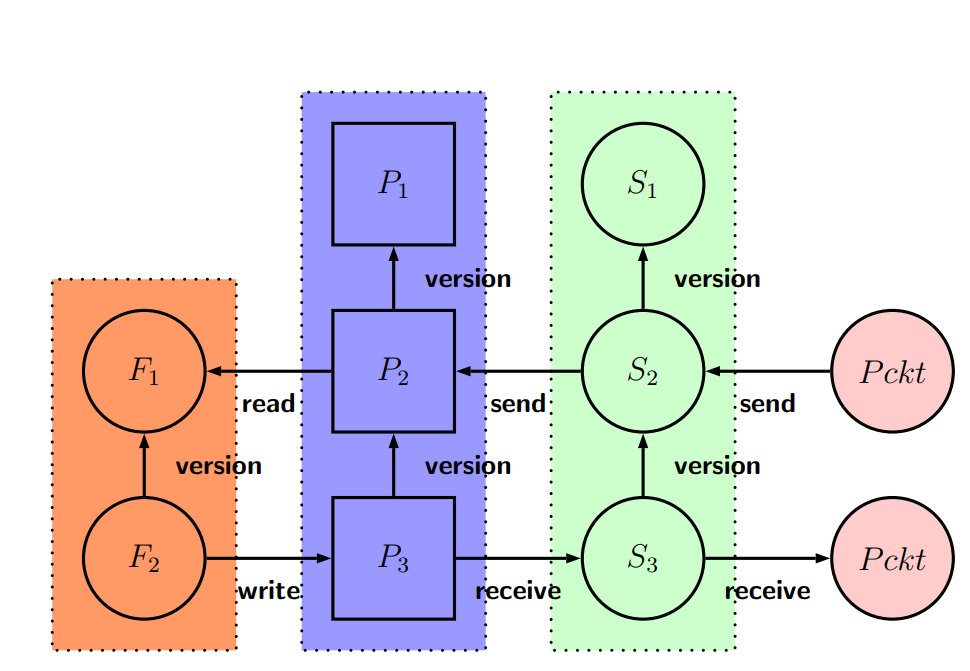
\includegraphics[width=0.7\linewidth]{provenance-g}
	\caption{An example of a provenance graph. CamFlow-Provenance partial graph example. A process P reads information from a file F, sends the information
		over a socket S, and updates F based on information received
		through S}
	\label{fig:provenance-g}
\end{figure}

\begin{figure}
	\centering
	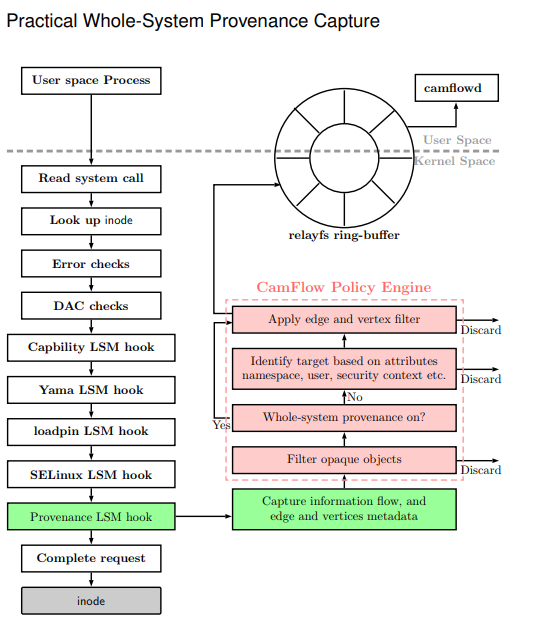
\includegraphics[width=0.7\linewidth]{provenance-capture}
	\caption[open system call]{Executing an open system call. In green is the capture mechanism. The pink is the provenance tailoring mechanism.}
	\label{fig:provenance-capture}
\end{figure}
\subsection{Provenance Data Model}
As explained in the previous sections according to W3C standards the provenance is defined as a directed acyclic graph(DAG). Fig 6 represents an example of a provenance graph. A process P reads information from a file F, sends the information
over a socket S, and updates F based on information received
through S.